\chapter{IdentityServer3}
\label{chap:IdentityServer3}
Prosjektgruppen begynte prosjektet med å se på mulig implementasjon av en løsning basset på rammeverket IdentityServer3. Dette vedlegge beskriver hvordan en implementasjon av autentiseringssystemet kunne sett ut om vi hadde bassert systemet på IdentityServer3.

\section*{Arkitekturvalg}
\label{sec:identityServer3_arkitekturvalg}
For å få et arkitekturisk overblikk over systemet brukes SAD fra RUP med Philippe Kruchten’s 4+1 view modell (se figur \ref{fig:4+1illustrasjonssikkse}). 4+1 tar utgangspunkt i at det overordnede use case diagrammet (se figur \ref{fig:OverordnetUseCase}) er definert. Det overordnede use case diagrammet regnes som '+1' av de '4+1' og befinner seg i midten av modellen (figur \ref{fig:OverordnetUseCase}). De fire views'ene som som ligger rundt senarioene i Use Caset har til hensikt å illustrere ulike synsvinkler inn mot senarioene (senarione er beskrevet i kapittel \ref{subsec:use_case_logge_inn}). Setter man alle delene av 4+1 modellen sammen kan man være relativt sikker på at de aller fleste av problemstillingene ved systemet i forhold til arkitektur blir dekt. 

\begin{figure}[H]
    \centering
    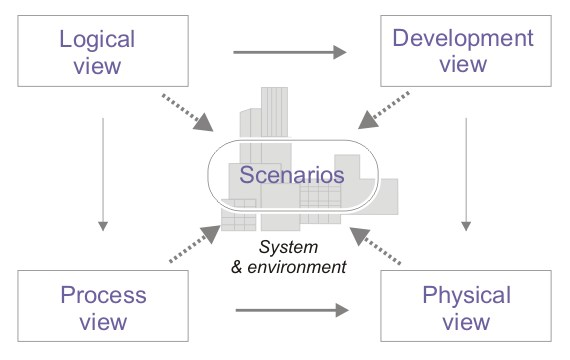
\includegraphics[scale=0.50]{graphics/04-arkitektur/4+1_Architectural_View_Model.jpg}
    \caption{4+1 illustrasjonsskisse. Hentet fra wikipedia}
    \label{fig:4+1illustrasjonssikkse}
\end{figure}

\section{Use case View}
\label{sec:use_case_view}
Vi har laget 4 extended use caser: logge inn, logge ut, glemt passord og egenadministrasjon. Ved å gjøre dette fikk vi større innblikk i det vi ser på som den viktigste funksjonaliteten.

\subsection{Logge inn}
\label{subsec:use_case_logge_inn}
\newline \textbf{Use case:} Logge inn på en webtjeneste
\newline \textbf{Aktør:}	Sluttbruker, Applikasjon og Azure AD
\newline \textbf{Mål:} Bruker skal kunne få tilgang til ønsket applikasjon. Applikasjon skal være sikker på at bruker har tilgang.
\newline \textbf{Beskrivelse:} Når bruker skriver inn brukernavn og passord skal brukeren autentiseres og få tilgang til applikasjonen den ønsker å jobbe på.
\newline \textbf{Pre-betingelser:} Bruker finnes allerede i systemet. 
\newline \textbf{Post betingelser:} Autentisert i alle webtjenester via Norkart ID.
\newline \textbf{Spesielle krav:} Har tilgang til NorkartID i nettverk eller via web.
\newline \textbf{Detaljert hendelsesforløp:}
\newline
\newline \textbf{Brukerhandling}
\newline 1. Use casen begynner når brukeren går til nettsiden for å bruke programmet.
\newline 2. Klient ber bruker om å  logge inn med brukernavn og passord.
\newline 3. Sluttbruker skriver inn innloggingsdetaljer.
\newline 4. Klient sender innloggings request til OpenID Connect
\newline 8. Bruker sender autentiseringskoden til OpenID Connect automatisk tilklienten.
\newline 9. Klient sender inn autentiseringskode for å motta token.
\newline 11. Token valideres i klienten.
\newline
\newline \textbf{Systemrespons}
\newline 5. OpenID Connect autentiserer sluttbruker mot Azure AD.
\newline 6. Azure AD autentiserer sluttbruker.
\newline 7. Norkart ID sender autentiseringskode til sluttbruker.
\newline 10. OpenID Connect sender en ID token og Access token til klienten (RP).
\newline

\begin{figure}[H]
    \centering
    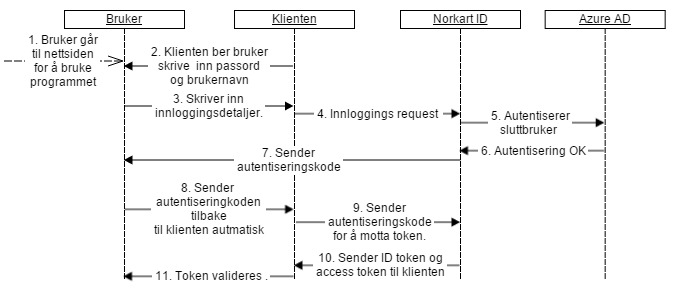
\includegraphics[scale=0.55]{graphics/04-arkitektur/UseCaseSekveknsdiagramLoggeInn.jpg}
    \caption{Sekvensdiagram 'logge inn'}
    \label{fig:skevensdiagramLoggInn}
\end{figure}

\noindent Figur \ref{fig:skevensdiagramLoggInn}, viser sekvensdiagrammet for når en bruker logger inn, og hvordan systemet kommer til å håndtere en slik spørring. Dette er en litt forenklet representasjon av hva som står under detaljert hendelsesforløp.
\newline
\newline
Nedenfor vises det ulike hendelsesforløp der det er bruker feil eller systemfeil.
\newline

\newline \textbf{Brukerfeil}
\begin{itemize}
\item Bruker skriver feil passord
\newline Bruker bes om å skrive brukernavn og passord på nytt og beskjed til bruker vil være: Innlogging feilet.
\item Bruker skriver feil brukernavn
\newline Bruker bes om å skrive inn brukernavn og passord på nytt og beskjed til bruker vil være: Innlogging feilet.
\item Gjentatt forsøk på innlogging med ugyldige opplysninger
\newline Bruker bes etter 5 forsøk om å vente 5 minutter før det prøves igjen. Skulle det igjen ikke gå går det 20 minutter til neste gang bruker kan prøve.
\end{itemize}

\bigskip \textbf{Systemfeil}
\begin{itemize}
\item Lang innloggingstid
\newline Om innloggings skulle ta mer enn 2 sekunder skal det gies beskjed til bruker at det tar unormalt lang tid å logge inn. Skulle det feile så bes bruker om å prøve en gang til. Om det skulle feile enda en gang til bes det om å ta kontakt med support, enten lokalt eller eksternt.
\item Innlogging ikke mulig å gjennomføre
\newline Skulle innlogging feile bes bruker om å prøve på nytt i første omgang. Om dette ikke skulle løse problemet bes bruker om å ta kontakt med support, enten lokalt eller eksternt.
\end{itemize}


\subsection{Logge ut}
\label{subsec:use_case_logge_ut}
\newline \textbf{Use case:} Logge ut via en webtjeneste
\newline \textbf{Aktør:}	Sluttbruker og Azure AD
\newline \textbf{Mål:} Bruker skal kunne få logget ut av ønsket applikasjon og fra alle andre tjenester.
\newline \textbf{Beskrivelse:} Når bruker klikker logg ut skal brukeren bli utlogget i alle systemet, både web, mobil og applikasjonsnivå. En singel-sign-out(for aktivt token) måte hvor man slipper å måtte logge ut individuelt i alle systemer.
\newline \textbf{Pre-betingelser:} Er allerede innlogget.
\newline \textbf{Post betingelser:} Blir logget ut i alle tjenester/sletter token slik at bruker er ute av alle webtjenester
\newline \textbf{Detaljert hendelsesforløp:}
\newline
\newline \textbf{Brukerhandling}
\newline 1. use casen begynner når brukeren går til tjenesten for å logge ut.
\newline 2. Bruker klikker logg ut.
\newline 3. Klient sender request til OpenID Connect.
\newline 5. Token blir slettet og viser i klienten at man har blitt logget ut.
\newline
\newline \textbf{Systemrespons}
\newline 4. OpenID Connect håndterer utloggings request og trigger utloggingskall til alle tjenester
\newline
\newline
Bruker kommuniserer med Norkart ID igjennom en klient som viser hvordan man skal gå frem for å kunne logge inn, se figur \ref{fig:skevensdiagramLoggUt}. Under ser du logge ut sekvensdiagrammet og hvordan det kommer til å bli:
\newline

\begin{figure}[H]
    \centering
    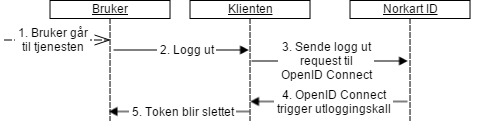
\includegraphics[scale=0.55]{graphics/04-arkitektur/UseCaseSekveknsdiagramLoggeUt.jpg}
    \caption{Sekvensdiagram 'logge ut'}
    \label{fig:skevensdiagramLoggUt}
\end{figure}

\textbf{Brukerfeil}
\begin{itemize}
\item Bruker logger ikke ut før han forlater arbeidsstasjonen
\newline Bruker bli automatisk logget ut etter et tidsintervall på 6 timer slik at om man skulle glemme å logge seg ut må man reautentisere seg når man returnerer.
\end{itemize}

\bigskip \textbf{Systemfeil}
\begin{itemize}
\item Bruker blir ikke logget ut av alle webtjenestene
\newline Bruker får beskjed om at det ikke var mulig å gjennomføre forespørsel og bes om å gå inn direkte på Norkart ID tjeneste og prøve på nytt. Om dette ikke skulle være nok skal det reises et flagg om at det er problem med utlogging.
\end{itemize}


\subsection{Glemt passord}
\label{subsec:use_case_glemt_passord}
\newline \textbf{Use case:} Glemt passord på websiden
\newline \textbf{Aktør:}	Sluttbruker, Azure AD og E-post
\newline \textbf{Mål:} Bruker skal kunne få mulighet sette nytt passord og få logget inn igjen.
\newline \textbf{Beskrivelse:} Bruker skal kunne hente ut passord selv til sin brukerprofil uten å måtte kontakte kundeservice. Her er tanken at man skal kunne motta en epost med en reset link hvor du kommer inn direkte til hvor du skal opprette nytt passord.
\newline \textbf{Pre-betingelser:} Bruker er allerede registrert med epostadresse.
\newline \textbf{Detaljert hendelsesforløp:}
\newline
\newline \textbf{Brukerhandling}
\newline 1. Use casen begynner når brukeren går til nettsiden få nytt passord.
\newline 2. Bruker klikker på glemt passord.
\newline 3. Bruker skriver inn epostadressen sin og bekrefter en captcha test.
\newline 7. Bruker blir bedt om å henvende seg til epost innboksen sin for å forsette.
\newline
\newline \textbf{Systemrespons}
\newline 5. Systemet slår opp bruker i databasen.
\newline 6. Det genereres en resetlink og den blir sendt til registrert epost.
\newline
\newline
Siden vi lager en singel-sign-in er det vel så viktig med en single-sign-out hvor du blir logget ut i alle tjenestene. Dette gjøres med tanke på sikkerhet og for å gjøre det lettere for bruker å kunne logge ut av systemet.
\newline
\newline
Nedenfor vises det ulike hendelsesforløp der det er bruker feil eller systemfeil.
\newline

\begin{figure}[H]
    \centering
    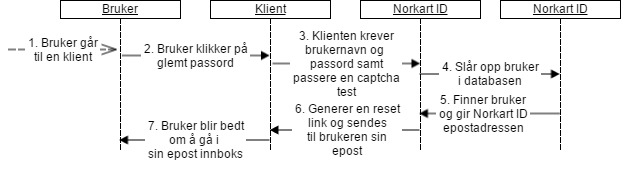
\includegraphics[scale=0.55]{graphics/04-arkitektur/UseCaseSekveknsdiagramGlemtPassord.jpg}
    \caption{Sekvensdiagram 'glemt passord'}
    \label{fig:skevensdiagramGlemtPassord}
\end{figure}

\noindent \textbf{Brukerfeil}
\begin{itemize}
\item Bruker oppgir ugyldig format på epost adresse
\newline Det gies en beskjed til bruker om at det er brukt feil format på epostadressen som er skrevet inn og presenterer a@b.c som format.
\item Bruker feiler på capcha sjekken
\newline Refresher siden 
\end{itemize}

\bigskip \textbf{Systemfeil}
\begin{itemize}
\item Epost blir ikke sendt ut.
\newline Det gjøres ingen sjekk av systemet annet enn at linken som blir sendt ut er gyldig i 30 minutter. Hvis den ikke kommer fram til bruker får bruker selv prøve på nytt.
\end{itemize}

\subsection{Egenadministrasjon}
\label{subsec:use_case_egenadministrasjon}
\newline \textbf{Use case:} Egenadministrasjon av brukerprofil
\newline \textbf{Aktør:}	Sluttbruker og Azure AD
\newline \textbf{Mål:} Bruker skal kunne endre på registrerte opplysning inne på sin brukerprofil.
\newline \textbf{Beskrivelse:} Når bruker er autentisert skal han kunne gå inn for å endre på sin profil. Det er her sluttbruker får tilgang til epost, telefon, generelle opplysning som er registrert. Brukeren har her mulighet til å endre de attributtene som går an og endre. Dette er en egen nettside hvor bruker får tilgang til etter autentisering.
\newline \textbf{Pre-betingelser:} Er allerede innlogget i systemet
\newline \textbf{Post betingelser:} Endringer skjer i sanntid og bruker og brukerprofil tar i bruk endringer i sanntid.
\newline \textbf{Detaljert hendelsesforløp:}
\newline
\newline \textbf{Brukerhandling}
\newline 1. Use casen begynner når brukeren går til nettsiden for å endre brukerdata.
\newline 2. Viser siden for egenadministrasjon.
\newline 4. Ved lagring kan bruker forsatt gjøre endringer eller logge ut.
\newline
\newline \textbf{Systemrespons}
\newline 3. Endringer gjort fra klient blir overført til database og klient.
\newline

\begin{figure}[H]
    \centering
    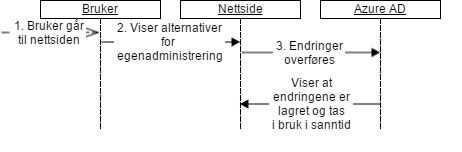
\includegraphics[scale=0.55]{graphics/04-arkitektur/UseCaseSekveknsdiagramEgenadministrasjon.jpg}
    \caption{Sekvensdiagram 'egenadministrasjon'}
    \label{fig:skevensdiagramEgenadministrasjon}
\end{figure}

\noindent Denne sees på som viktig for å kunne muliggjør noen form for selvadministrering til brukerne som igjen resulterer til mindre trykk på Norkart kundeservice.
\newline
\newline Nedenfor vises det ulike hendelsesforløp der det er bruker feil eller systemfeil.
\newline
\newline \textbf{Brukerfeil}
\begin{itemize}
\item Ikke innlogget
\newline Bruker skal bli henvist til innloggingssiden når bruker ikke har valid token eller ikke er innlogget.
\item Endrer til ugyldig informasjon i brukerprofilen
\newline Når bruker endrer opplysninger skal disse sjekkes ved hjelp av enten Javascript sjekker eller biblioteker for å klient sjekke at informasjonen riktig skrevet før den går inn i systemet. 
\end{itemize}

\bigskip \textbf{Systemfeil}
\begin{itemize}
\item Om systemet ikke klarer å behandle endringsforespørsel
\newline Systemet skal gi beskjed tilbake om endringer er OK eller ikke. Ved tilfeller der det ikke er OK bes bruker å prøve på nytt og hvis feilen vedvarer om å ta kontakt med Norkart.
\end{itemize}

\section{Logisk View}
\label{sec:logisk_view}
I forhold til 4+1 modellen har det logiske viewet til hensikt å illustrere sluttbrukers perspektiv på produktet. For å øke skalerbarheten og sikkerheten til systemet er det brukt en trelags arkitektur hvor Model View Controller (MVC) er brukt som arkitekturpattern i det øverste laget. MVC er brukt for å skape mindre avhengigheter i systemet og for å redusere kodekompleksiteten. For å få en oversikt over lag og klasser er det utviklet et design klassediagram, se figur \ref{fig:LogiskViewKlassediagram}.

\begin{figure}[H]
    \centering
    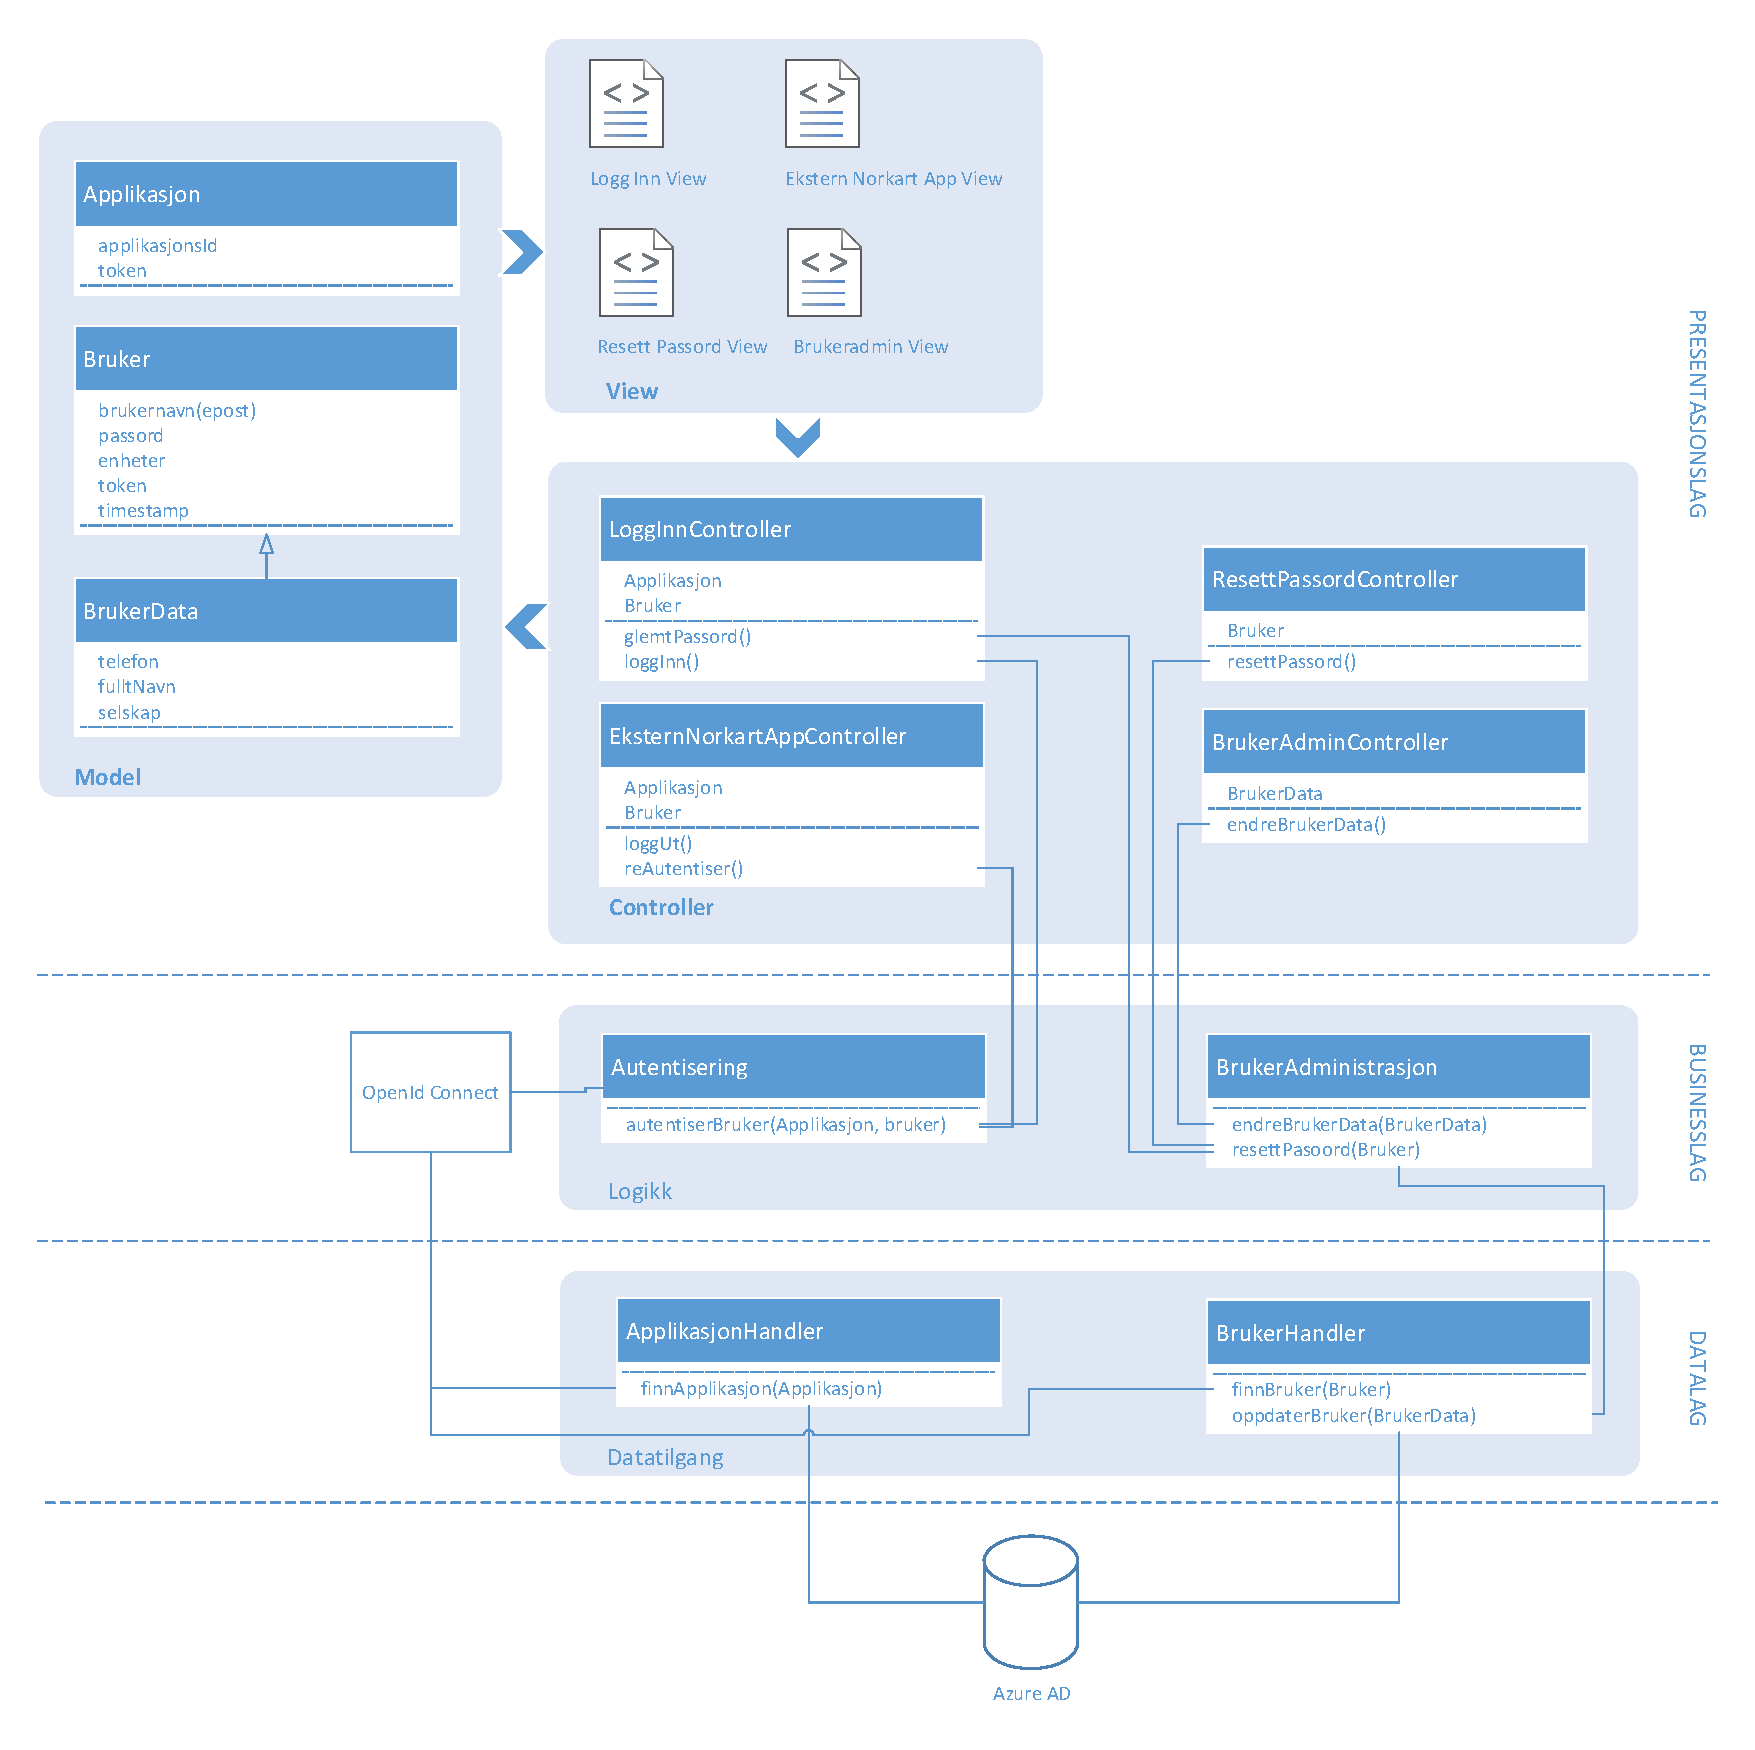
\includegraphics[scale=0.45]{graphics/04-arkitektur/LogiskViewKlassediagram}
    \caption{Klassediagram}
    \label{fig:LogiskViewKlassediagram}
\end{figure}

\subsection*{Trelagsarkitektur}
\label{subsec:logisk_view_trelagsarkitektur}
Klassediagrammet (se figur \ref{fig:LogiskViewKlassediagram}) viser at systemet er delt opp i et trelagssystem. Et trelagssystem muliggjør at hvert lag kan oppgraderes eller skiftes ut individuelt. Slik blir det billigere og enklere å endre systemet hvis det blir forandringer i kravene, eller det dukker opp ny teknologi som kan være mer hensiktsmessig å bruke. Lagene som er brukt er presentasjonslag, businesslag og datalag. Under står det beskrevet hva de tre lagene har ansvar for og hva de inneholder.
\newline
\subsection{Presentasjonslag}
\label{subsec:logisk_view_presentasjonslag}
Presentasjonslaget består av brukergrensesnittet og har som hovedmål å videreformidle input fra brukeren til resten av systemet og oppdatere brukergrensesnittet når input er behandlet. Det er bygd opp av et MVC pattern med fire views og fire tilhørende controllere. Systemet har i tillegg tre modell klasser.
\newline

\subsubsection{Views}
\label{subsec:logisk_view_views}
Viewene viser data til sluttbruker. Hvert view har sin controller som videreformidler input fra bruker nedover i arkitekturen.
\newline
\begin{itemize}
\item Logg Inn View
\newline Inneholder en glemt passord link og et logg inn skjema.
\item Ekstern Norkart App View
\newline En ekstern Norkart applikasjon brukere har logget seg inn på via Norkart ID. Her finnes en logg ut knapp.
Resett Passord View
\item Dette viewet inneholder muligheten til å resette passord. \newline Sluttbruker kan kun komme til dette viewet fra en link motatt i e-post under glemt passord funksjonalitet.
\item Egenadmin View
\newline Inneholder et skjema med brukerdata som brukeren kan endre på og oppdatere.
\end{itemize}

\bigskip
\subsubsection{Controllere}
\label{subsec:logisk_view_controllere}
Controllere informerer model og view om endrigner basert på input fra bruker. Klassediagrammet (se figur \ref{fig:LogiskViewKlassediagram}) viser hvilke klasser de forskjellige controllerne tilkaller på forskjellig input.
\newline
\begin{itemize}
\item Logg inn Controller 
\newline Starter glemt passord funskjonalitet og informerer businesslaget om at bruker vil logge seg inn.
\item Ekstern Norkart App Controller
\newline Setter i gang logg ut funskjonalitet. 
\item Resett Passord Controller
\newline Sier fra til businesslaget at bruker ønsker å resette sitt passord.
\item Egenadmin Controller 
\newline Sender ny brukerdata nedover i systemet for å oppdatere bruker.
\end{itemize}

\bigskip
\subsubsection{Modeller}
\label{subsec:logisk_view_modeller}
Systemet har tre modeller som brukes til å holde på data.
\newline
\begin{itemize}
\item Bruker
\newline Inneholder brukerens autentiserings data.
\item BrukerData
\newline Er et barn av bruker modellen og inneholder brukerens administrative data.
\item Applikasjon
\newline Inneholder applikasjonsdata til bruk i autentiseringsprosessen.
\end{itemize}

\subsection{Businesslag}
\label{subsec:logisk_view_buisnesslag}
Businesslaget har ansvar for logikken i systemet og mottar henvendelser fra presentasjonslaget. Det snakker også med klassene i datalaget for hendvendelser mot Azure AD. Systemet har to hovedklasser som styrer logikken i systemet.
\newline
\begin{itemize}
\item Autentisering
\newline Har ansvar for all logikken som må gjøres for at en bruker skal autentiseres mot sine applikasjoner.
\item EgenAdministrasjon
\newline Utøver all logikk som skal til for endring og oppdatering av bruker data.
\end{itemize}

\subsubsection{OpenID Connect}
\label{subsubsec:logsik_view_buisnesslag_openid_connect}
I tillegg til de to logikk klassene vil også OpenID Connect ligge i businesslaget. OpenID Connect brukes for å autentisere brukere.

\subsection{Datalag}
\label{subsec:logsik_view_datalag}
\labe{subsec:datalag}
Datalaget har ansvaret for alle henvendelser mot AzureAD og består av to hovedklasser.
\newline
\begin{itemize}
\item ApplikasjonHandler
\newline Sjekker om applikasjoner eksitsterer i Azure AD
\item BrukerHandler
\newline Sjekker om brukere eksisterer og oppdaterer brukerdata  i Azure AD
\end{itemize}

\section{Prosess View}
\label{sec:prosess_view}
\newline Som prosess view har vi valgt å lage activity diagram for de 4 overordnede use casene (se kapittel \ref{sec:use_case_view}). Activity diagram har til hensikt å illustrere arbeidsflyt, etter hendelser og valg når en oppgave skal gjennomføres. Vi har valgt å lage activity diagrammer for de fire kjerne funksjonene prosjektet initielt skal fokusere på.
\newline
\newline Begrepet applikasjonsserver1 brukes for å illustrere servere som kjører applikasjoner NorkartID autentiserer og autoriserer brukere for.
\newline

\subsection{Logge ut}
\label{subsec:prosess_view_logge_ut}
Activity diagram “Logge ut” (figur \ref{fig:ProsessViewLoggeUt}) begynner når en bruker sender en forespørsel til NorkartID serveren om å logge ut. For å kunne logge ut må brukeren bekrefte at det faktisk er brukeren som ønsker og logge ut. Dette gjøres for å beskytte mot at angripere kan kaste ut brukere fra  applikasjonene de er logget inn på. Avhengig av måten applikasjoner er koblet opp mot Norkart ID vil utgangsverdiene etter diagrammet ende opp i tre ulike tilstander. 

\begin{figure}[H]
\centering
    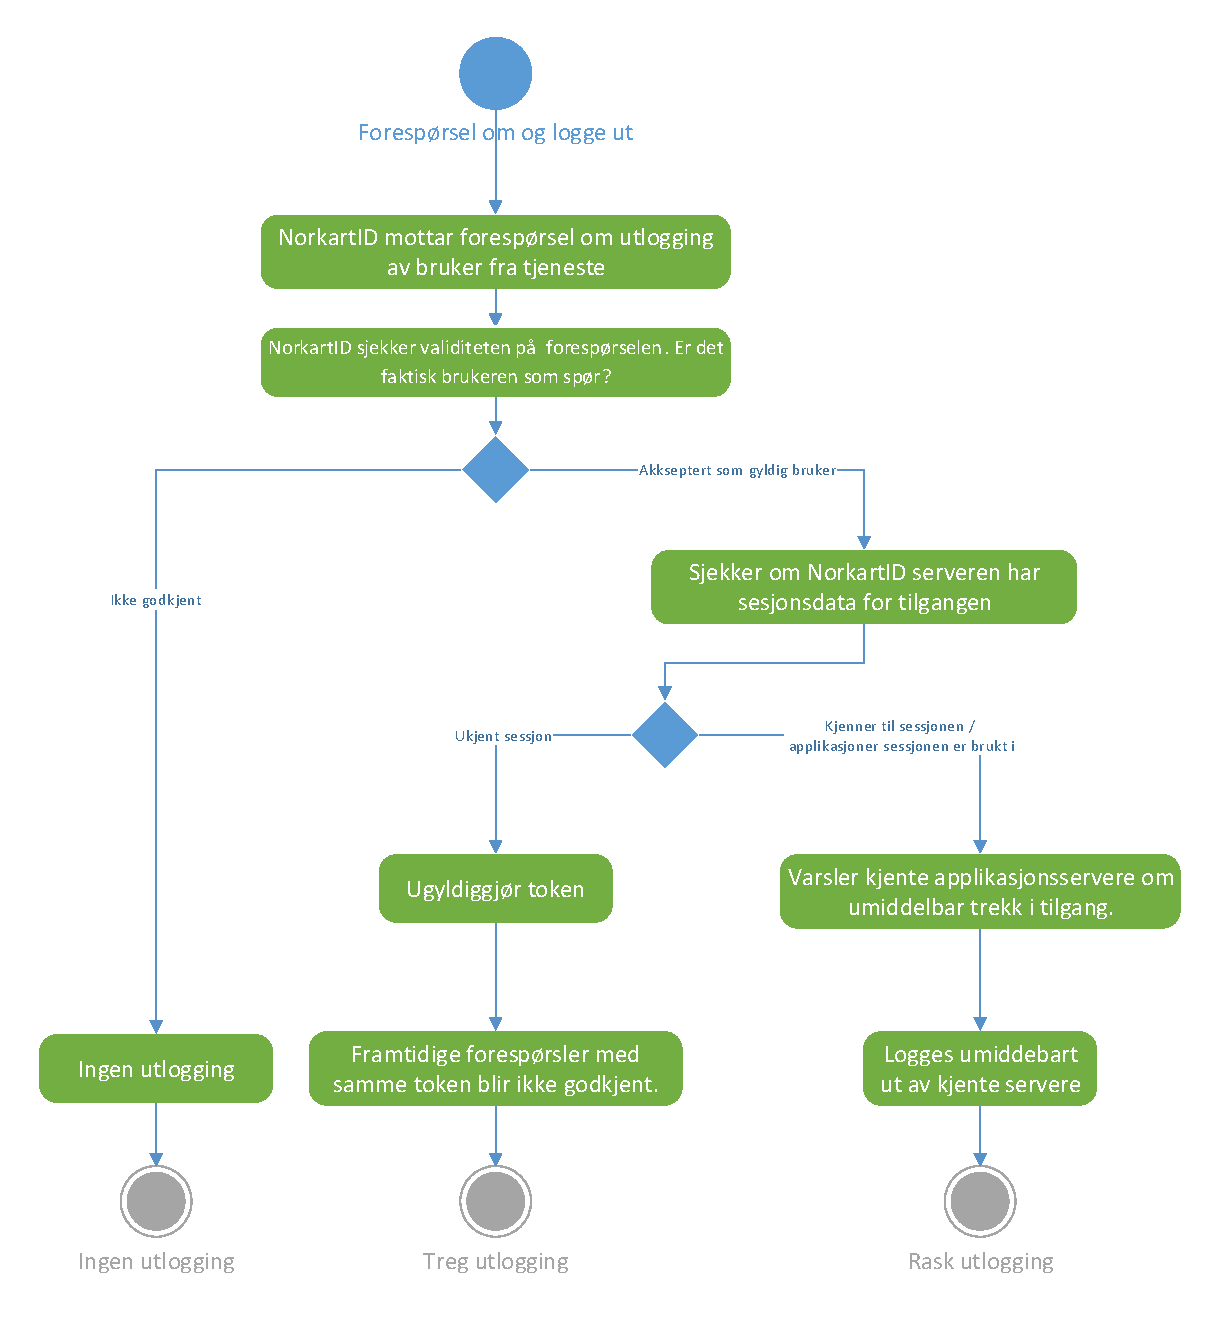
\includegraphics[scale=0.65]{graphics/04-arkitektur/ProsessViewLoggeUt}
    \caption{Activity diagram 'logge ut' }
    \label{fig:ProsessViewLoggeUt}
\end{figure}

\subsubsection*{Kommentar}
\label{subsubsec:prosess_view_logge_ut_kommentar}
Vi ser for oss at det kun er applikasjoner som støtter rask-utlogging fra applikasjon serveren som får lov til å dele access-token med andre prossesser. For de applikasjonene som kun støtter treg utlogging, anbefales bruk av egen access token, uten mulighet for å dele denne access token med andre applikasjoner. Dette vil føre til en egen pålogging før bruk, men vil øke sikkerheten bruker og Norkart. I oppgaven kommer vi ikke til å fokusere på denne problemstillingen innledende, men vil forsøke å dokumenter dette på best mulig måte for å gi Norkart grunnlag for en sikrest mulig bruk av tjenesten når på sikt tar systemet i bruk.
\newline

\subsection{Logge inn}
\label{subsec:prosess_view_logge_inn}
Activity diagramet påloggingsforespørselen (figur \ref{fig:ProsessViewLoggeInn}) begynner inngangsverdien etter at en bruker har sendt inn brukernavn og passord for å logge på en spesifikk tjeneste. Utgangsverdiene fra diagrammet er at brukeren blir logget inn eller avvist. Activity diagrammet tar ikke hensyn til eventuellt sikkerhets mekanismer som er lagt inn for å hindre brute-force pålogging på serveren. Dette vil vi likevel forsøke å implementere mekanismer mot, og vil trolig bygges inn som en del av de to første hendelsene etter inngangsverdien i diagrammet.
\newline

\subsection{Glemt passord}
\label{subsec:prosess_view_glemt_passord}
Activity diagrammet “glemt passord” (figur \ref{fig:ProsessViewGlemtPassord}) begynner etter at en bruker har skrevet inn en brukerid, muligens bekreftet at det faktisk er en bruker som forsøker å resette passordet, og ikke en datamaskin igjennom en captcha test. Prosessen innebærer at det sendes en mail til bruker som bruker må bekrefte innen 30 min for at resettingen av passordet skal være godkjent. Dersom samme bruker klikker på glemt passord flere ganger i løpet av en halvtime, uten og bekrefte på mail i mellomtiden, vil det kun være den siste mailen som ble sendt fra serveren som faktisk vil gi mulighet til å resette passordet. Eldre mail fra serveren vil da ugyldiggjøres. 
\newline

\subsection{Egenadministrasjon}
\label{subsec:prosess_view_egenadministrasjon}
Activity diagram “Egenadministrasjon (figur \ref{fig:ProsessViewEgenadministrasjon}) brukes for å illustrere når en bruker selv kan gjøre endringer av egne brukerprofildata. Inngangsverdien er at bruker skal logge inn på for å endre, første handling er at bruker logger på id.norkart.no. Vi forutsetter at dette fører til en vellykket innlogging. Utgangsverdien er at brukeren, enten bruker har endret brukerprofildata eller ikke, logger ut, eller forlater id.norkart.no.
\newline

\begin{figure}[H]
\centering
    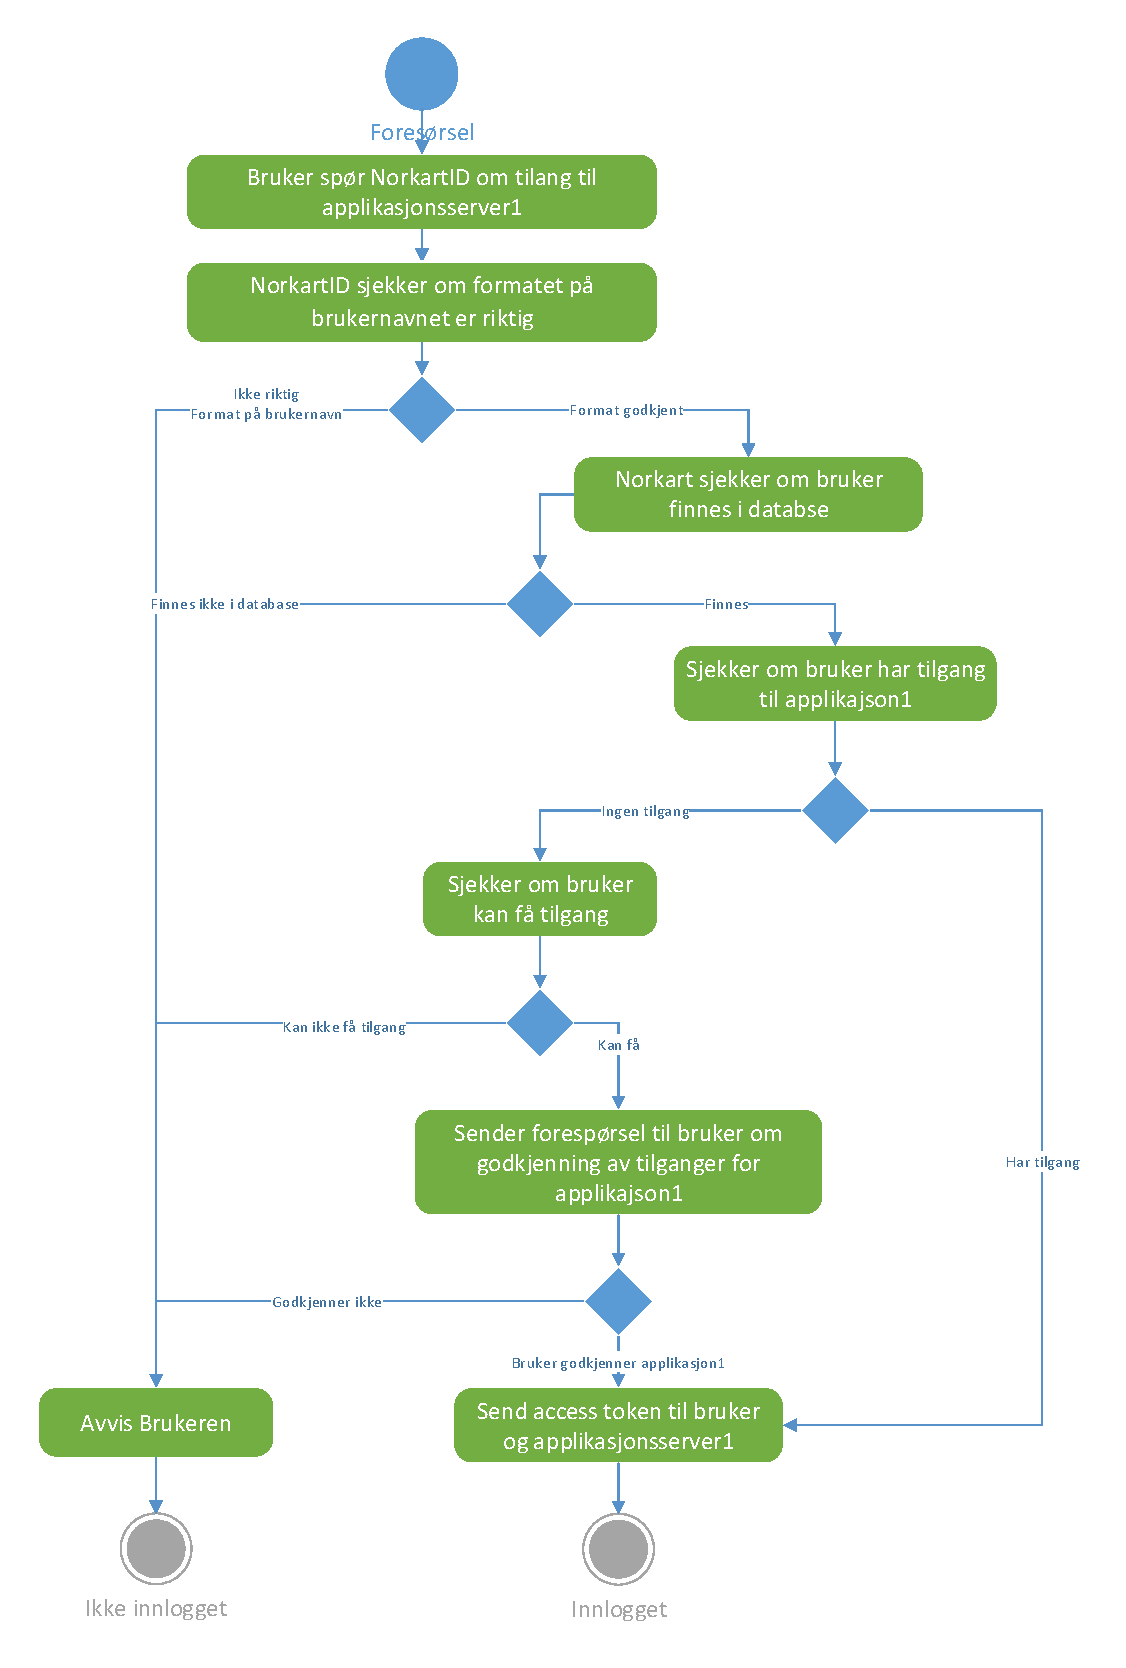
\includegraphics[scale=0.65]{graphics/04-arkitektur/ProsessViewLoggeInn}
    \caption{Activity diagram 'logge inn' }
    \label{fig:ProsessViewLoggeInn}
\end{figure}

\begin{figure}[H]
\centering
    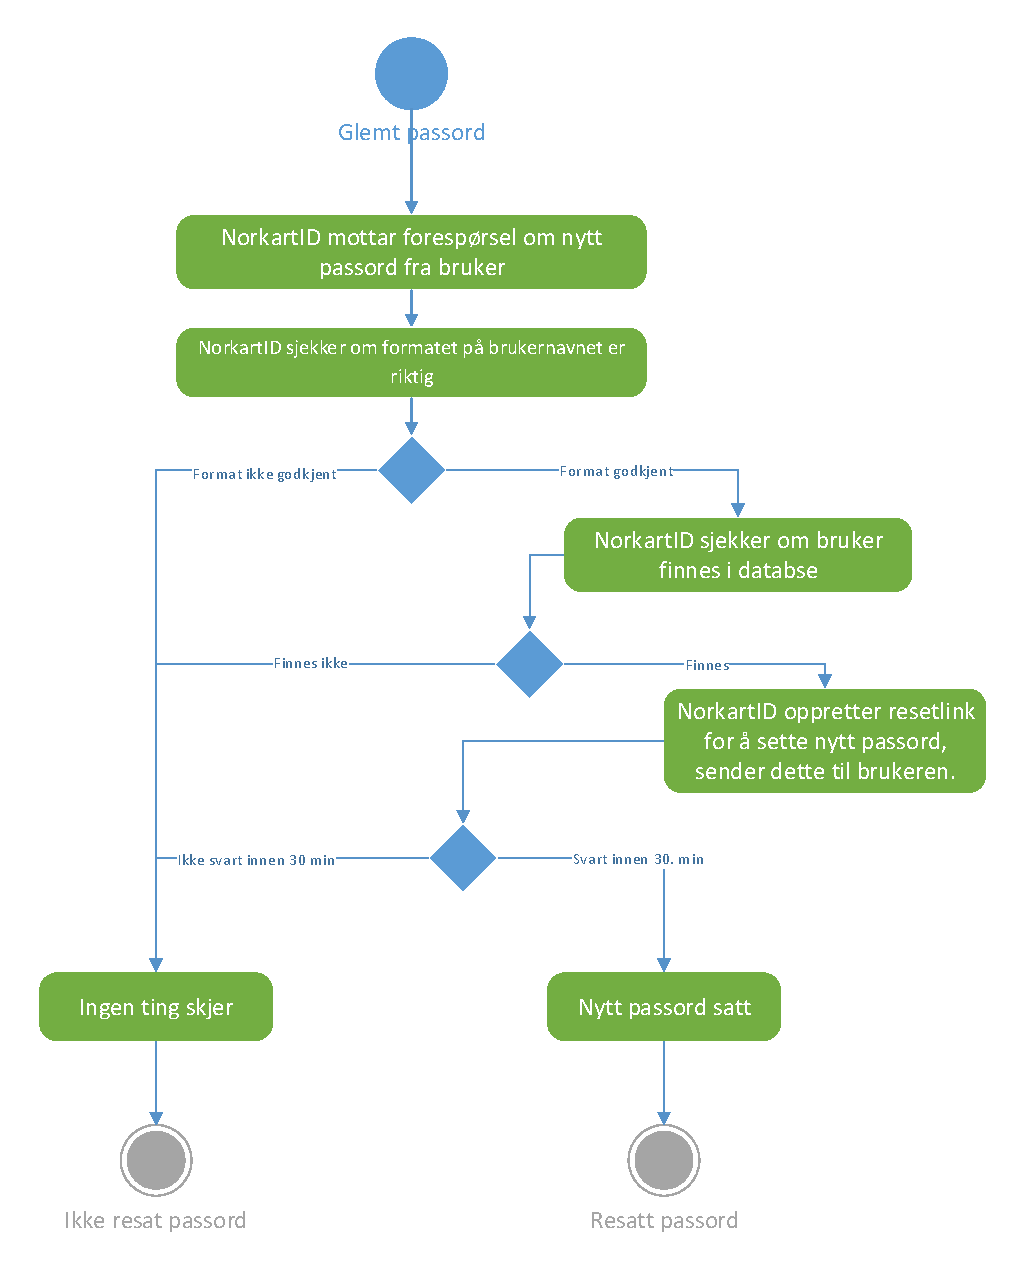
\includegraphics[scale=0.65]{graphics/04-arkitektur/ProsessViewGlemtPassord}
    \caption{Activity diagram 'glemt passord' }
    \label{fig:ProsessViewGlemtPassord}
\end{figure}

\begin{figure}[H]
\centering
    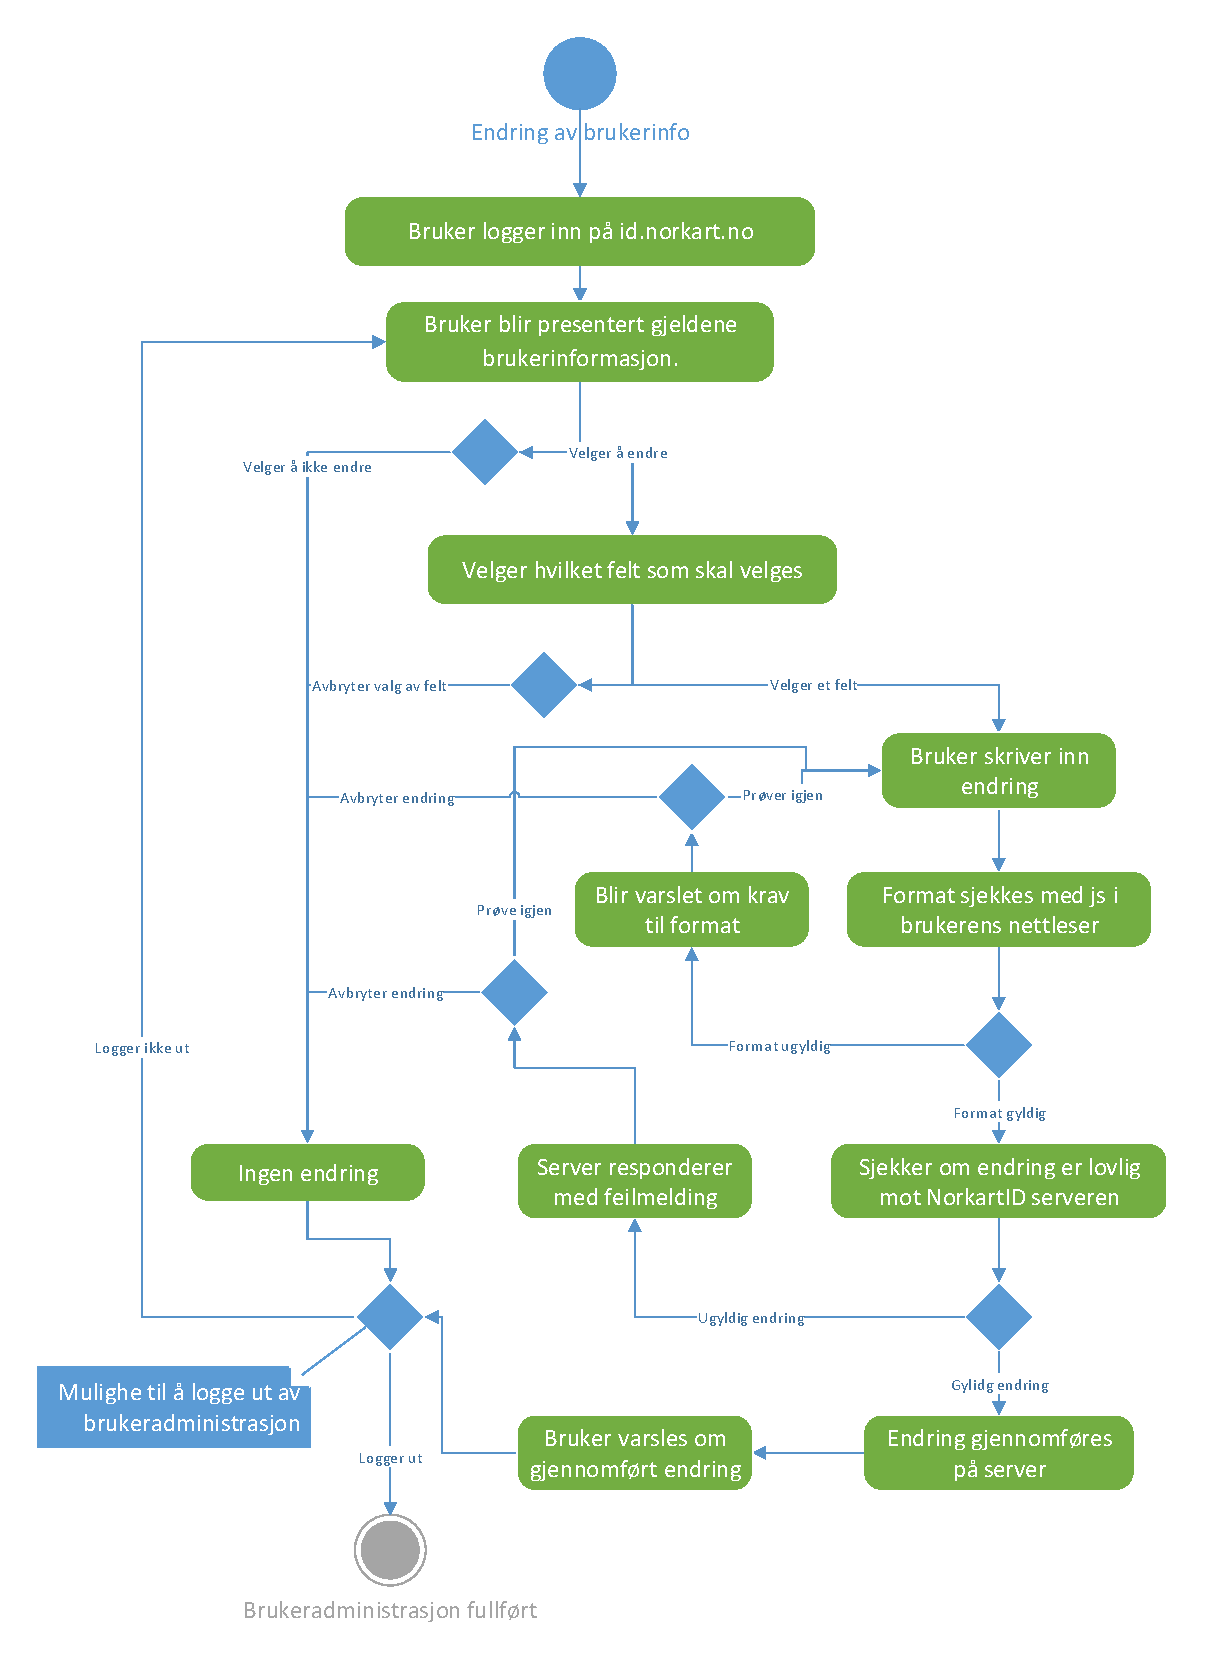
\includegraphics[scale=0.65]{graphics/04-arkitektur/ProsessViewEgenadministrasjon}
    \caption{Activity diagram 'egenadministrasjon' }
    \label{fig:ProsessViewEgenadministrasjon}
\end{figure}

\section{Utviklings View}
\label{sec:utviklings_view}
Dette viewet har til hensikt å illustrere systemet fra en programmerers perspektiv. Dette er gjort ved å lage et komponent diagram, se figur \ref{fig:UtviklingsViewDevelopmentView}. Systemet består av flere komponenter som er avhengig av hverandre for å fungere. For å kunne bruke systemet er webserveren avhengig av Norkart ID. Norkart ID vil fungere som hovedkomponent. For å kunne logge inn og autentisere brukere er Norkart ID avhengig av OpenID Connect for autentisering og en Azure AD for å finne brukere og hvilke applikasjoner disse har tilgang til. Norkart ID er i tillegg avhenig av en Azure AD for å administrere brukere. Hvis en bruker har glemt sitt passord må Norkart ID kontakte en epost server.  Norkart ID inneholder i tillegg to komponenter, nemlig Bruker Administrasjon og Autentisering. Bruker Administrasjon er avhengig av at brukeren er autentisert for å kunne utføre sine oppgaver.

\begin{figure}[H]
    \centering
    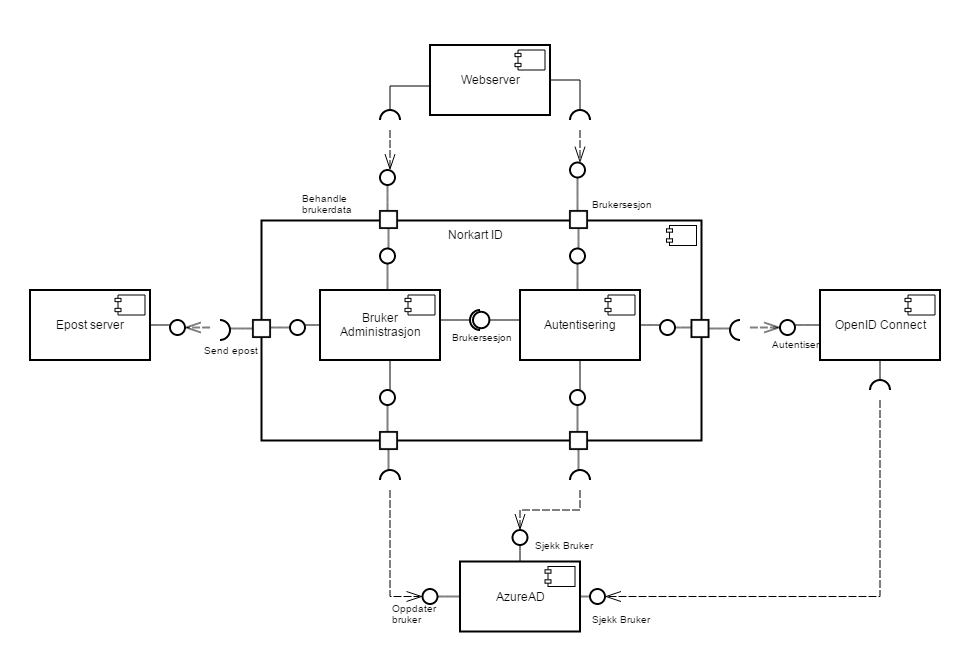
\includegraphics[scale=0.40]{graphics/04-arkitektur/UtviklingsViewKomponentDiagram.png}
    \caption{Komponent diagram over Norkart ID }
    \label{fig:UtviklingsViewKomponentDiagram}
\end{figure}

\section{Distribusjons View}
\label{sec:distribusjons_view}
AHensikten med distribusjons view er å illustrere hvordan systemet skal settes opp i forhold til hardware implementasjon. Ettersom hele Norkart ID er planlagt å kjøre på virituelle maskiner i Norkart sin nettsky, illustrerer vi bare distribusjons view med tre elementer i distribusjons diagrammet (se figur \ref{fig:UtviklingsViewDistribusjonsDiagram}). Vi regner Bruker som en betegnelse på brukere av systemet.  Applikasjoner i diagrammet er de applikasjonene Norkart ID skal gi brukeren tilgang til, altså de Norkart ID skal autentisere og autorisere tilganger for. Den markerte rammen rundt "Azure AD" og "Norkart ID med OpenID Connect" skal illustrere at systemet ligger virituelt på en sky. Når applikasjoner ligger utenfor skyen betyr dette bare at det stilles ingen krav til at applikasjonene må være en del av den samme skyen, eller kjøre på de samme serverene. 

\begin{figure}[H]
    \centering
    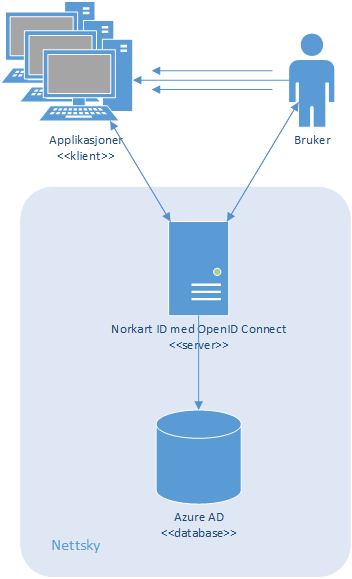
\includegraphics[scale=0.55]{graphics/04-arkitektur/UtviklingsViewDistribusjonsDiagram.png}
    \caption{Distribusjons diagram for Norkart ID }
    \label{fig:UtviklingsViewDistribusjonsDiagram}
\end{figure}